\documentclass[a4paper]{jacow}

\usepackage[utf8]{inputenc}
\usepackage[USenglish]{babel}			 
\usepackage[final]{pdfpages}
\usepackage{multirow}
\usepackage{ragged2e}
\usepackage{amsmath}
\usepackage{tikz}

\begin{document}

\title{Investigation of Nature Inspired Algorithms in a practical context by exploiting the characteristics of Braitenberg Vehicle Concepts}

\author{A. Dorn\thanks{andrea.dorn@uni-rostock.de}, University of Rostock, Rostock, Germany \\
		H. Pommerenke\thanks{hermann.pommerenke@uni-rostock.de}, University of Rostock, Rostock, Germany \\
		T. Steinmetz\thanks{tino.steinmetz@uni-rostock.de}, University of Rostock, Rostock, Germany}
	
\maketitle


\begin{abstract}
   Insert shiny abstract!
\end{abstract}

\section{The Braitenberg Vehicle}
The term Braitenberg Vehicle is used to describe a vehicle, which is able to move autonomously only by considering primitive sensor inputs (e.g. proximity, gas or light sensors). It also includes two independent controllable motors and two biases, one for each motor, to ensure a continuous motor movement in case that the vehicle reaches a position, where all sensor inputs become zero.

The values collected by the sensors are weighted and superimposed for each motor individually, whereby the symmetry characteristics of the sensor positions can be exploited, i.e. the weight vector of the first motor can be turned upside down to fit the second motor. Equation~\ref{eq:motorequation} represents this principle, where the index $n$ describes the number of the motor and $i$ the number of the individual sensor.

\begin{equation}
	V_{Motor,n} = V_{Bias,n} + \sum\limits_{i=0}^{N-1}w_{n,i}\cdot V_{Sensor,i}
	\label{eq:motorequation}
\end{equation}

For this project the educational robot e-puck is used to serve as a Braitenberg Vehicle. It holds eight proximity sensors, which can be used for the above mentioned sensor inputs. Figure~\ref{fig:epuck} shows the symmetric distribution of the sensors and the basic principle of the motor control.

\begin{figure}[hbt]
	\centering
	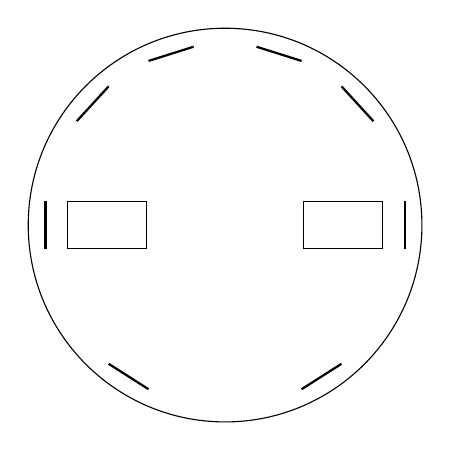
\begin{tikzpicture}
		\draw (0,0) circle [radius=2.5];
		\draw (1,-0.3) rectangle (2,0.3);
		\draw (-1,-0.3) rectangle (-2,0.3);
		\draw [thick](-7.5:2.3) -- (7.5:2.3);
		\draw [thick](35:2.3) -- (50:2.3);
		\draw [thick](65:2.3) -- (80:2.3);
		\draw [thick](100:2.3) -- (115:2.3);
		\draw [thick](130:2.3) -- (145:2.3);
		\draw [thick](172.5:2.3) -- (187.5:2.3);
		\draw [thick](230:2.3) -- (245:2.3);
		\draw [thick](295:2.3) -- (310:2.3);
	\end{tikzpicture}
	\caption{Sketch of the e-puck robot, with motors, sensors and weights}
	\label{fig:epuck}
\end{figure}

The autonomous behaviour of the Braitenberg Vehicle can now be explained with a simple example. Imagine the robot is determined to avoid obstacles. If sensor one registers an approaching obstacle and therefore generates a value, motor one will begin to reduce it's speed, while motor two will begin to speed up, which results in turning the whole robot to the left.

\end{document}
	